\chapter{Návrh}
\label{sec:de}

\section{Návrhový vzor MVC}
\label{sec:de_mvc}

Struktura nadřazeného systému je vhodná k~použití návrhového vzoru MVC, tedy \textit{model-view-controller}. \textit{Model} zde představují garáže (podřízené systémy), k~nim vázané události a logika jejich vyhodnocování. 

\textit{View} je zobrazení těchto dat, tedy především generované HTML stránky webového rozhraní. Jako další \textit{view} je možné považovat získávání dat (například ve formátu JSON) pomocí API nadřazeného systému, třeba při zasílání registračních klíčů podřízeným systémům.

\textit{Controller} je pak část aplikace, která se stará o~zpracování HTTP požadavků. Ty mohou přicházet jednak z~uživateloval prohlížeče, jednak od podřízených systémů. Na základě těchto požadavků pak \textit{controller} posílá příslušné příkazy \textit{modelu}. Struktura aplikace při použití vzoru MVC je naznačena na obrázku \ref{fig:mvc}.

\begin{figure}[h!]
    \centering
    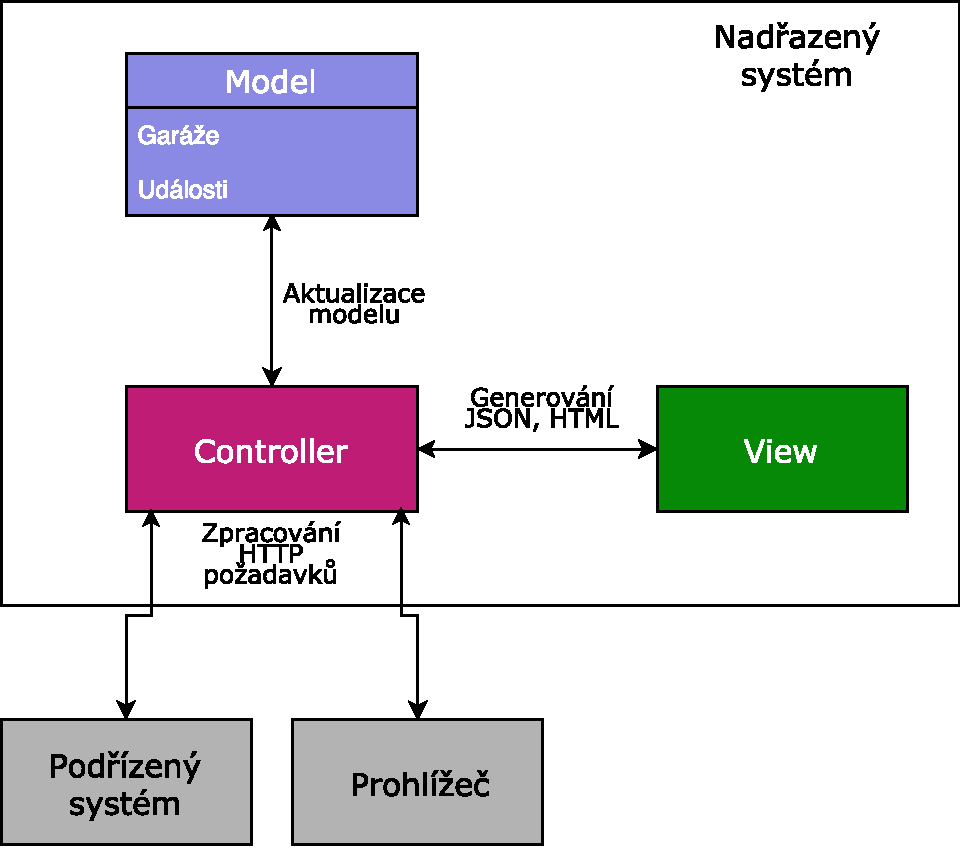
\includegraphics[width=0.7\textwidth]{images/mvc.pdf}
    \caption{Struktura MVC aplikace}
    \label{fig:mvc}
\end{figure}

Hlavní motivací pro použití tohoto vzoru je snadná rozšiřitelnost. Pokud by například bylo potřeba aplikaci doplnit o~komunikaci s~podřízenými systémy pomocí MQTT, stačí pouze vytvořit vhodný \textit{controller}. Ten pak může využívat \textit{model} aplikace stejným způsobem jako HTTP \textit{controller}.

Tento návrhový vzor popisuje pouze nadřazený systém spravující garáže. Kromě toho je součástí aplikace ještě autentizace uživatele při přístupu do uživatelského rozhraní. Tuto funkci jsem se rozhodl pojmout jako samostatnou komponentu, popsanou v~sekci \ref{sec:de_auth}.

\section{\textit{Model}}

\textit{Model} představuje jádro nadřazeného systému. Je zde implementována vnitřní reprezentace uchovávaných dat, což jsou především zaznamenané události. Každá událost má také svého původce, tedy garáž (přesněji podřízený systém v~této garáži).

Kromě toho \textit{model} implementuje \textit{business logiku} sytému, tedy například vytváření nových garáží (registraci podřízených systémů) či reakce na příchozích události.

Ostatní části aplikace (\textit{view} a \textit{controller}) používají \textit{model}, bez znalosti jeho vnitřní struktury, pomocí následujících operací:

\begin{itemize}
    \item \textbf{Vytvoření garáže} -- registrace nového podřízeného systému. V~případě vytváření pomocí API (tj. přímo podřízeným systémem) vyžaduje operace zapnutý registrační mód. Pokud je nová garáž vytvářena ve webovém rozhraní, registrační mód není vyžadován.
    \item \textbf{Editace garáže} -- například změna označení.
    \item \textbf{Smazání garáže} -- smazáním garáže dojde k~odstranění zaznamenaných událostí a zneplatnění příslušného API klíče.
    \item \textbf{Zapínání/vypínaní registračního módu}.
    \item \textbf{Přístup k~uloženým datům} -- obecně operace typu získání všech garáží nebo událostí vázané ke konkrétní garáži.
    \item \textbf{Vytvoření události} -- základní požadavek využívaný podřízenými systémy.
\end{itemize}

Vnitřně pak model na základě těchto operací autentizuje pomocí API klíčů požadavky podřízených systému, validuje zaslaná data a spravuje databázi systému.

\subsection{Garáž -- \texttt{Garage}}

Třída \texttt{Garage} reprezentuje konkrétní podřízený systém a uchovává s~ním spojená data:

\begin{itemize}
    \item \texttt{id} -- identifikace entity v~databázi.
    \item \texttt{tag} -- uživatelem zvolené označení garáže. To slouží pro snadnější orientaci ve webovém rozhraní (uživatel nemusí garáže rozlišovat podle nic neříkajícího \texttt{id}).
    \item \texttt{api\_key} -- klíč umožňující přístup k~API systému. Ten je také zaslán zařízení při jeho registraci.
    \item \texttt{last\_report} -- datum a čas posledního kontrolního hlášeí.
    \item \texttt{next\_report} -- datum a čas dalšího očekávaného hlášení.
    \item \texttt{period} -- perioda kontrolních hlášení.
    \item \texttt{state} -- stav garáže (otevřeno/zavřeno).
    \item Seznam událostí spojených s~touto garáží.
\end{itemize}

\subsubsection{Vytváření nových garáží}

Nové garáže mohou v~systému vznikat dvěma způsoby. První možnost je vytvoření nové garáže přímo v~uživatelském rozhraní. Po vytvoření se zde zobrazí vygenerovaný API klíč, který je potřeba nahrát na příslušný podřízený systém. Způsob nahrávání by závisel na příslušném hardwaru (například sériová linka). Tato možnost je určena především pro podřízené systémy, které by nepodporovaly zaslání registračního požadavku a nevyžaduje zapnutý registrační mód.

Druhá možnost je použít registrační mód. V~tom případě je nová garáž vytvořena na základě registračního požadavku podřízeného systému. Vygenerovaný API klíč je při tom zaslán jako odpověď na požadavek, a není tedy nutné ho ručně nahrávat. Registrační mód je možné aktivovat v~uživatelském rozhraní. Pokud mód není aktivovaný, nadřazený systém odmítne všechny požadavky na registraci.

\subsection{Událost -- \texttt{Event}}

Třída \texttt{Event} představuje událost zaznamenanou podřízeným systémem. Jak bylo zmíněno v~sekci \ref{sec:de_mvc}, jsou tyto události vázány ke konkrétním garážím, kdy každá událost má jednoznačně určeného původce, a každá garáž libovolné množství událostí.

Nadřazený systém rozlišuje dva druhy událostí. Kontrolní (plánované) události slouží ke kontrole funkčnosti podřízených systémů. Tyto události jsou odesílány v~pravidelném intervalu, určeném nadřazeným systémem. Ten v~odpovědi na požadavek s~kontrolní událostí zašle očekávaný čas (počet minut) do dalšího hlášení. Kontrolní událost nezasílá žádná data, funguje pouze jako známka života podřízeného systému.

Kromě kontrolních hlášení mohou podřízené systémy vytvářet mimořádné události. Mimořádná událost nastane při překročení mezních hodnot některého z~čidel (tedy detekce kouře, pohybu či otevření/zavření dveří).

Základní třída \texttt{Event} a podtřídy \texttt{CheckEvent} a \texttt{SensorEvent} obsahují tyto údaje:

\begin{itemize}
    \item \texttt{id} -- identifikace entity v~databázi.
    \item \texttt{timestamp} -- časové razítko.
    \item Garáž, která je původcem události.
    \item \texttt{CheckEvent} dále obsahuje:
        \begin{itemize}
            \item \texttt{next\_report} -- datum a čas dalšího očekávaného hlášení.
        \end{itemize}
    \item \texttt{SensorEvent} dále obsahuje:
        \begin{itemize}
            \item \texttt{type} -- typ senzoru.
            \item \texttt{value} -- naměřená hodnota ????
        \end{itemize}
\end{itemize}

eventuelne napsat ze ta trida \texttt{SensorEvent} bude mit podtridy podle typu senzoru, ze to bude lepsi kvuli rozsiritelnosti. To uvidim co se mi bude vic libit az to zkusim naimplementovat

\subsubsection{Vyhodnocení události}

\subsection{Fasáda}

\section{Controller}

Flask API

\subsection{API}

dulezita je idempotence prikazu, tj. bude prikaz na udalost votevreno a na udalost zavreno ale ne toggle, aby se nerozbil stav garaze na serveru.

\section{View}

\section{Autentizace uživatele}
\label{sec:de_auth}

tady budou takovy ty veci jako kde je ulozeny heslo, hashovani hesel a tak

plus teda to ze je to zvlast vod toho nadrazenyho systemu, tzn tady urcite bude pouzitej ten blueprint

este teda napsat ze vsechny ty veci spojeny s~uzivatelem nebudou ulozeny v~ty databazi ale jen v~nakym konfiguraku (veci jako heslo a pripadne ten notifikacni mail)
